\documentclass[11pt]{article}
\setlength{\topmargin}{0in}
\setlength{\headheight}{0in}
\setlength{\headsep}{0in}
\setlength{\textheight}{8.7in}
\setlength{\textwidth}{6.5in}
\setlength{\oddsidemargin}{0in}
\setlength{\evensidemargin}{0in}
\setlength{\parindent}{0.3in}
\setlength{\parskip}{0.10in}

\special{papersize=8.5in,11in}
\setlength{\pdfpageheight}{\paperheight}
\setlength{\pdfpagewidth}{\paperwidth}

\usepackage{graphicx}
\usepackage{subfig}

\begin{document}

\title{Glacial cycles during the past three million years}
\author{Miles Wu}
\maketitle

\begin{abstract}
abs
\end{abstract}

\section{Introduction}
%how to measure ice volumes
The global ice volume can be inferred from looking at what is called the `$\delta^{18}$O' of sediment cores.
Deep sea sediment cores have foraminifera shells of calcium carbonate (chemical formula: CaCO$_3$).
Although oxygen most commonly has an atomic mass of $16$ ($99.8\%$), there is a less common but stable isotope with an atomic mass of $18$ ($0.2\%$) \cite{viu}.
In `$\delta^{18}$O' analysis we look at the ratio of these two stable isotopes in the carbonates in the sediment cores.
It has been found that during glacial periods the cores have a high $\delta^{18}$O' value.
As a result we can use these to infer the global ice volume as it is proportional to the $\delta^{18}$O' value.

%explain
This correlation between global ice volume and $\delta^{18}$O value can be explained.
The lighter $^{16}$O isotope moves slightly faster as it is lighter and therefore it evaporates slightly more frequently than the heavier isotope.
As a result water vapor is slightly $^{16}$O-enriched and it leaves the sea from which it evaporated slightly $^{18}$O-enriched.
The largest amount of evaporation takes place near the equator so it becomes heavier and this water vapor moves towards the poles where it rains and therefore the polar waters become lighter.
This Rayleigh fractionation becomes more pronounced the larger the global ice volume, as the ice at the polar regions store the lighter isotope from the polar seas \cite{viu}.

%so what are the phenomenon
Looking at these cores, geoscientists found that appearance of northern continental glaciers occurred at around three million years ago \cite{fedorov}.
This is thought to be well understood as just the conclusion of a longer gradual cooling trend \cite{huybers}.
However, after the onset of glaciation, the last three million years have had a dramatic increase in fluctuations, especially in ice volume.
This can be seen in Figure \ref{d18o}; the important thing to note is that the scale along the horizontal axis changes at $t=3~\textnormal{Ma}$ and therefore the fluctuations are significantly larger in amplitude.

% paper topic
The reason for the sudden onset of these severe glacial cycles and their patterns are a topic of present debate.
Hyubers provides a plausible explanation for the timing of the cycles and does some statistical analysis to justify his explanation \cite{huybers}.
He further goes on and provides a simple model to describe the cycles.
Philander and Barreiro also propose a modification to Huybers' simple model.
In this paper we look at these two papers, comparing and contrasting their respective models.

\begin{figure}
  \centering
  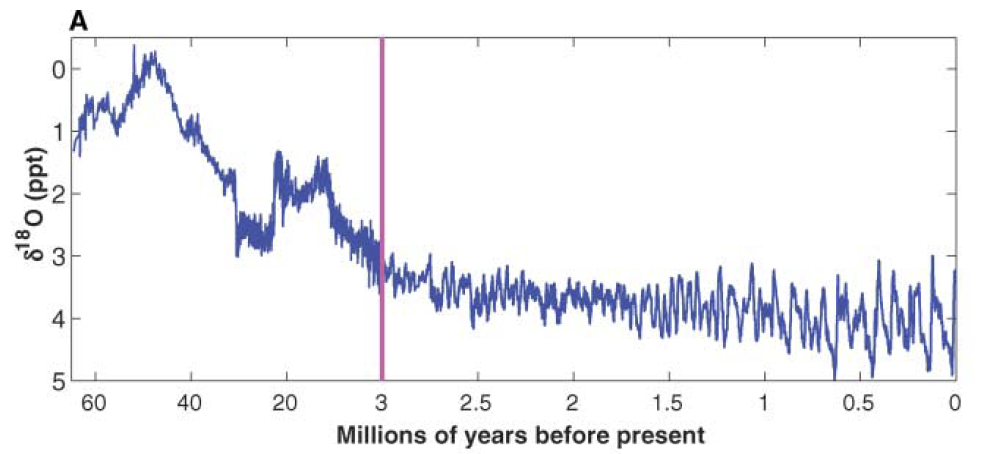
\includegraphics[width=4in]{d18o.png}
  \caption{cap}
  \label{d18o}
\end{figure}

\section{Milankovitch Forcing}
%region definitions
In Figure \ref{d18o} there is another change around approximately $1.2~\textnormal{Ma}$, where the fluctuations in the global ice volume become even more abrupt and violent.
This change is known as the mid-Pleistocene transition.
We use this to split up the past three million years into two regions: the earlier calmer region from 3 Ma to 1.2 Ma and the later more violent region from 1.2 Ma to the present.
Let us examine the former region first.

%no disagreement about first part
Huybers, after analyzing these early pleistocene glacial cycles using Fourier transforms and spectral analysis, reports that these have a period of approximately forty thousand years \cite{huybers}.
Philander and Barreiro also report a similar thing, saying that there are oscillations with a period of forty-one thousand years \cite{philander}.
Both explain this through a phenomenon known as Milankovitch forcing, in particular the obliquity forcing, as this cycles in the phenomenon has a forty-one thousand year cycle; this seems a very reasonable explanation as it would be unlikely that it was a coincidence that they share the same period to within a small amount of uncertainty.

%what is Milankovitch forcing
Milankovitch forcing is the name given to climate forcing by the Earth's orbit.
There are three parameters of our orbit around the sun: eccentricity, obliquity and precession.
Eccentricity is a variable that relates the shape of the Earth's orbit relative to a circular orbit, obliquity is the tilt of the earth, and precession is the change in direction of the earth's rotation axis.
These three parameters are constantly changing and their cycles affect how much sunlight falls on the Earth and its glaciers, which in turn can influence glaciation or deglaciation rates through its warm rays.
Eccentricity has a one hundred thousand year period, precession a nineteen thousand and a twenty-three thousand year period and obliquity a forty-one thousand year period, so it makes a lot of sense to attribute the glacial cycles to obliquity cycles as it seems plausible that it could affect glacier rates \cite{uri}.

In the later region (1.2 Ma to the present) spectral analysis yields a different picture.
No longer is there a peak at forty thousand years, but instead there is a broad peak at one hundred thousand years \cite{huybers}; this change in cycle periods is a distinguishing feature of this second region compared to the first.
The cycles are actually either approximately eighty thousand years or one hundred thousand years and so the two peaks of the spectral analysis plot have just merged \cite{philander}.
Because the cycles are multiples of the obliquity cycle (forty thousand years) both Huyberr and Philander and Barreiro agree that the glaciation cycles are still controlled by the obliquity \cite{hyubers}\cite{philander}.
There are other possible explanations stemming from eccentricity or precessions, but Huybers points out that eccentricity does not have a big enough effect to cause the glaciation cycles and precession forcing is anti-symmetric between the hemispheres but the glacial cycles are symmetric \cite{hyubers}.
Attributing the cycles to obliquity seems reasonable and the reasons that Huybers puts forward for why it can't be other phenomenon seem plausible too. 

%statistical test?
While it seems pretty conclusive for the first region (3 Ma to 1.2 Ma), it is not quite so obvious and clear-cut for the second region (1.2 Ma to the present); some kind of quantitative method is needed to justify the argument.
As a result, Huybers performs a statistical test as evidence for the validity of his explanation\cite{huybers}. 
His formal hypothesis is that deglaciations are triggered at a specific point in the phase of the obliquity cycle, and conversely his null hypothesis is that they are independent of the phase of obliquity and therefore should be uniformly distributed with respect to obliquity phase.
Deglaciation events are identified from the $\delta^{18}$O record as large changes and thirty-six events are found: twenty from the first period and sixteen from the second.
The results from this statistical test are quite conclusive as Hyubers finds that it is significant at the $99\%$ level for both the early and the late period.
This is also shown in a plot in Figure~\ref{hypotest}; the deglaciation events (red dot) are not uniformly distributed with respect to the obliquity phase (the large circle).

\begin{figure}
  \centering
  \subfloat[Early Pleistocene]{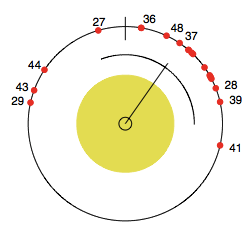
\includegraphics[width=2in]{hypotestc.png}}
  \subfloat[Late Pleistocene]{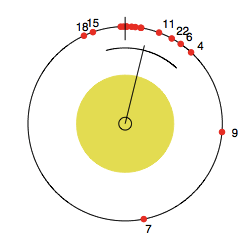
\includegraphics[width=2in]{hypotestd.png}}
  \caption{cap}
  \label{hypotest}
\end{figure}

%conclusion for this section
Obliquity cycles setting the pace for the glacial cycles is pretty convincing from the evidence presented by both Huybers and Philander and Barreiro.
Not only is it an explanation that makes sense and seems plausible, the statistical evidence from Huybers is very strong and is sufficient for us to conclude that obliquity is the root pacemaker for the glacial cycles.
Occam's razor is also another motivation for why obliquity cycles should be the cause of the glacial cycles in both the late and early Pleistocene.
This principle of science prefers the simpler explanation (less assumptions) for any given explanation of a phenomenon.
Here it is simpler that there is just one unified explanation and theory for glacial cycles that lasts throughout both periods, rather than two independent theories for each period, which would require another explanation for the transition too.

\section{Obliquity cycle skipping}
One mystery still remains: the glacial cycles in the late Pleistocene period do not match up with the obliquity cycles one-to-one and are some multiple of the forty-one thousand period.
Although we have shown that the deglaciation occurs at the same point in the obliquity cycle, we have not explained why it does not happen every cycle and usually one or two cycles are skipped in the late Pleistocene period.

Hyubers offers a simple model to explain this phenomenon.   

%difference in model with philander

%parameters of philander

%chaotic

\section{Conclusion} 



\begin{thebibliography}{9}
	\bibitem{huybers}
		I
	\bibitem{fedorov}
		I
    \bibitem{philander}
        I
	\bibitem{viu}
		I%chttp://web.viu.ca/earle/geol-412/oxygen%20Isotope%20fractionation.pdf
    \bibitem{uri}
        I%http://deschutes.gso.uri.edu/~rutherfo/milankovitch.html
\end{thebibliography}

\end{document} 